% !TeX spellcheck = cs_CZ
%{\tikzset{external/prefix={tikz/FYZII/}}
% \tikzset{external/figure name/.add={ch12_}{}}
%---------------------------------------------------------------------------------------------------
% file fey2ch12.tex
%---------------------------------------------------------------------------------------------------
%=========================== Kapitola: Analogie elektrostatiky =====================================
\setchaptertoc
\chapter{Analogie elektrostatiky}\label{fyz:IIchapXII}

  \section{Stejné rovnice mají stejné řešení}\label{fyz:IIchapXIIsecI}
  \section{Proudění tepla. Bodový zdroj v blízkosti nekonečného rovinného 
  rozhraní}\label{fyz:IIchapXIIsecII}
  \section{Napnutá membrána}\label{fyz:IIchapXIIsecIII}
  \section{Difúze elektronů. Kulově symetrický zdroj v homogenním 
  prostředí}\label{fyz:IIchapXIIsecIV}
  \section{Bezvírové proudění kapaliny. Obtékání koule}\label{fyz:IIchapXIIsecV}
  \section{Osvětlení. Homogenní osvětlení roviny}\label{fyz:IIchapXIIsecVI}
  \section{\uv{Fundamentální jednotka} přírody}\label{fyz:IIchapXIIsecVII}
  \section{Příklady a cvičení}\label{fyz:IIchapXIIsecVIII}


    \begin{figure}[ht!] %\ref{fyz:fig724}
      \centering
      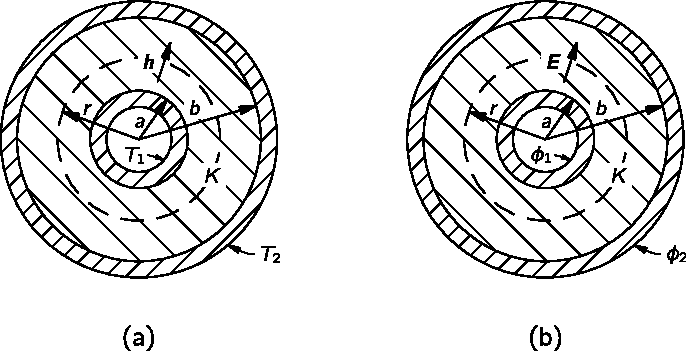
\includegraphics[width=0.7\linewidth]{fyz_fig724.pdf}
      \caption{
               (\cite[s.~707]{Feynman02})}
      \label{fyz:fig724}
    \end{figure}

    \begin{figure}[ht!] %\ref{fyz:fig725}
      \centering
      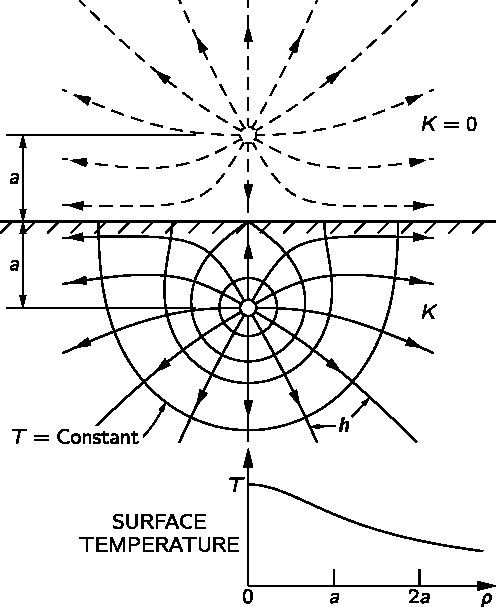
\includegraphics[width=0.7\linewidth]{fyz_fig725.pdf}
      \caption{
               (\cite[s.~707]{Feynman02})}
      \label{fyz:fig725}
    \end{figure}

    \begin{figure}[ht!] %\ref{fyz:fig726}
      \centering
      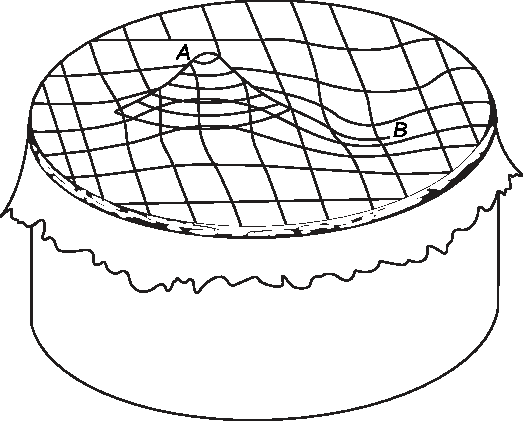
\includegraphics[width=0.7\linewidth]{fyz_fig726.pdf}
      \caption{
               (\cite[s.~707]{Feynman02})}
      \label{fyz:fig726}
    \end{figure}

    \begin{figure}[ht!] %\ref{fyz:fig727}
      \centering
      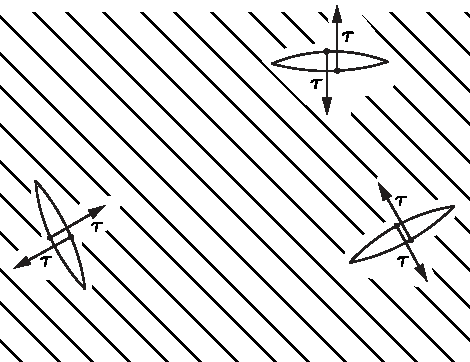
\includegraphics[width=0.7\linewidth]{fyz_fig727.pdf}
      \caption{
               (\cite[s.~707]{Feynman02})}
      \label{fyz:fig727}
    \end{figure}

    \begin{figure}[ht!] %\ref{fyz:fig728}
      \centering
      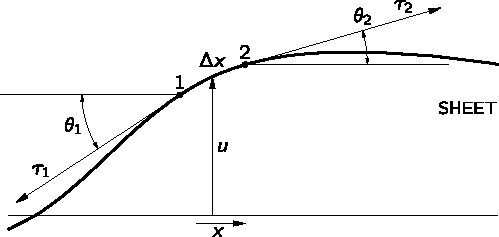
\includegraphics[width=0.7\linewidth]{fyz_fig728.pdf}
      \caption{
               (\cite[s.~707]{Feynman02})}
      \label{fyz:fig728}
    \end{figure}

    \begin{figure}[ht!] %\ref{fyz:fig729}
      \centering
      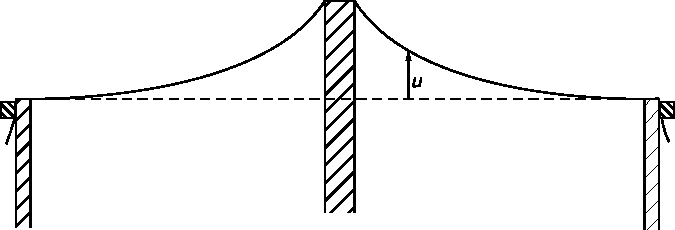
\includegraphics[width=0.7\linewidth]{fyz_fig729.pdf}
      \caption{
               (\cite[s.~707]{Feynman02})}
      \label{fyz:fig729}
    \end{figure}

    \begin{figure}[ht!]
      \centering
      \subcaptionbox{\label{fyz:fig730a}}{\luafigure[0.6]{fyz_fig730a.pdf}}               \newline
      \subcaptionbox{\label{fyz:fig730b}}{\luafigure[0.6]{fyz_fig730b.pdf}}
      \label{fyz:fig730}
      \caption{
               (\cite[s.~748]{Feynman02})}
    \end{figure}

    \begin{figure}[ht!] %\ref{fyz:fig731}
      \centering
      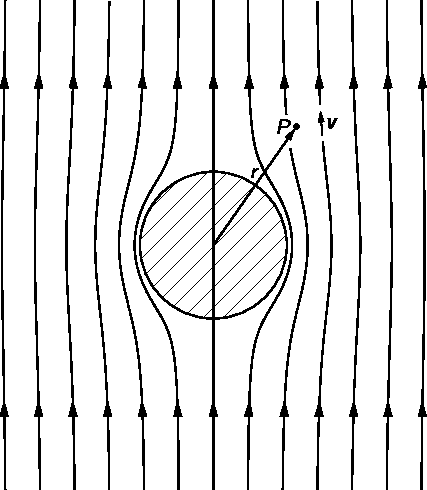
\includegraphics[width=0.7\linewidth]{fyz_fig731.pdf}
      \caption{
               (\cite[s.~707]{Feynman02})}
      \label{fyz:fig731}
    \end{figure}

    \begin{figure}[ht!] %\ref{fyz:fig732}
      \centering
      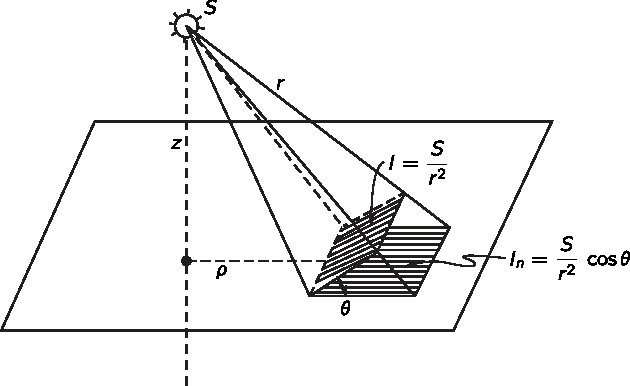
\includegraphics[width=1\linewidth]{fyz_fig732.pdf}
      \caption{
               (\cite[s.~707]{Feynman02})}
      \label{fyz:fig732}
    \end{figure}

\todo[inline]{Kapitola fey2c12 je nedodělaná, obsahuje pouze obrázky}
%} %tikzset
%---------------------------------------------------------------------------------------------------
